\documentclass{article}

\usepackage[utf8]{inputenc} %most IDEs use UTF8
\usepackage[T1]{fontenc} %most fonts needs T1
\usepackage{amsmath}
\usepackage{graphicx}

\begin{document}
\begin{titlepage}
    \begin{center}
        \vspace*{1cm}
        \Huge
        \textbf{A novel method to briefly localize the human movement on a flat surface}

        \vspace{1.5cm}


        \vspace{1.5cm}
        \LARGE
        \textbf{Zili Li}

        \vfill

        Script Not final version.

        \vspace{0.8cm}
        \normalsize

        National Engineering Research Center for E-Learning\\
        Central China Normal University\\
        China \\
        2024--06

    \end{center}
\end{titlepage}
\begin{abstract}
    This article propose a novel approach to localize human's movement on a flat surface using a fixed monocular camera. Assuming the person is moving on a flat surface and during the movement the person is not obscured by opaque objects.By solving a constrained perspective-3-point problem and filter the results using a modified Kalman filter.We can extract the localized movement information from the frames.
\end{abstract}
\section{Pinhole Camera Model} 
The pinhole camera model first introduced by Brunelleschi in the early fifteenth century provides a simple representation of how light interacts with a camera to form an image. The camera is represented as a simple opaque box with a tiny hole on one side and a flat plane on the opposite. All rays of light are blocked by the walls of the box except those passing through the tiny hole.
When an object is placed in front of the hole, rays of light reflecting or emitting from different points of the object pass through the hole to form an inverted image on the image plane. If Without the opaque box and the pinhole, every point on the plane would be illuminated from all points emitting or reflecting light from the object or the environment. Hence, the points on the image plane will be illuminated uniformly and no image can be observed.

\begin{figure}[h!]
    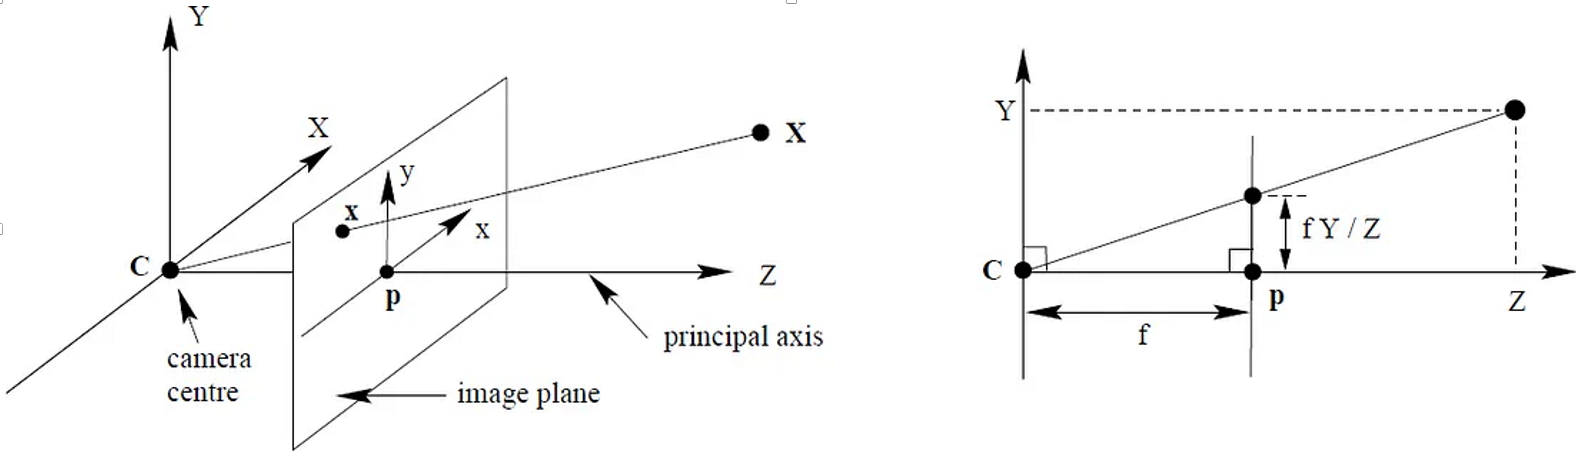
\includegraphics[width=\linewidth]{fig1.1.png}
    \caption{The pinhole camera model}\label{fig:1.1}
\end{figure}

The fig1.\ref{fig:1.1} represents the operating principle of the pinhole camera.

Objects farther away from the camera appear smaller in the image. The distance from the small hole to the image plane determines the field of view of the camera. A closer distance to image plane results in a smaller field of view, capturing more of the scene the image size of the distant object is proportional to the distance from the pinhole aperture to the image plane.

However, a real pinhole camera cannot work in most conditions since a small hole cannot let through enough light in an acceptable exposure time. Optical lens can gather much more light and however lens introduced optical distortions and aberrations to the image, making edge of the image sometimes unusable and corrections needed to restore properties of the image such as straight lines and color.

\section{The coordinate systems}
Here we must talk about the coordinates of the world coordinate and camera coordinates before we can give any meanful mathematical representations of out problem.

The parameters of the camera intrinsic matrix are estimated by performing the camera calibration procedure. The latter is typically performed using a set of known geometric patterns (e.g., chessboard patterns) or objects with precisely measured dimensions, allowing for the estimation of the camera parameters through mathematical algorithms, such as Zhang's method or the Direct Linear Transform (DLT) algorithm.
Coordinates represent locations of points under a given coordinate system. Since the world is big and ambiguous we shall not try to find a origin of the world but to change it to some where we feel comfortable with. That's why the transforms kicks in we need to know the coordinate of something under different coordinate systems.

In the view of camera everything is pixels, and the camera locates pixels by camera coordinate $(u,v)$(1) the origin is at upper left corner.

In the view of perspective transformation the origin of the camera locates at the principle
point$(x,y)$ and the world coordinate's origin locates at the focal point$(X_c,Y_c,Z_c)$ (3) share axis with the camera.
In the view of other stuff in the world, it has it's own coordinate and their own axis.(4)
\section{Camera Parameters}
\subsection[short]{The camera matrix}
The differences between different cameras can be described in these quantities:  

1. The focal length: The distance between the center of the projection and the image plane.

2. The center of projection: The point where the pinhole aperture is located against the image plane.

3. The optical axis is the line perpendicular to the image plane and passing through the center of projection.

4. The principal point is defined as the point of intersection between the optical axis and the image plane.

The focal length together with the sensor size determines the field of view and the magnification of the camera. A longer focal length results in a narrower field of view and magnifies distant objects, while a shorter focal length captures a wider field of view but diminishes the magnification of distant objects. Sensor size is the inverse of the focal length. Larger sensor is the same as we get shorter focal length smaller sensor is the same as we get longer focal length. We cannot determine the focal length just by measuring the size of items in the image.But for a know size of sensor it is possible.

The relation between a point \begin{equation}
    Q=(X, Y, Z)
\end{equation}in the real space and its projection on the image plane at the pixel location \begin{equation}
    (x_s, y_s)
\end{equation} is represented by the following equations:
\begin{eqnarray}
    x_s=f_x\frac{X}{Z}+c_x \\
    y_s=f_y\frac{Y}{Z}+c_y
\end{eqnarray}

where $c_x$and $c_y$
are two parameters that handle possible misalignment of the principal point with the center of the image; $f_x$ and $f_y$
are essentially the focal lengths expressed in pixels. We introduce two new parameters because each pixel on a typical image plane is rectangular, hence the pixel lengths in x and y are different. It is worth noting that $x_s,y_s,c_x,c_y,f_x,f_y$are expressed in units of pixels.The physical focal length f, usually expressed in units of millimeters, cannot be measured directly. However, the focal lengths $f_x$ and $f_y$ can be measured using a procedure called camera calibration.
4. Camera Intrinsic Matrix
Projective transform is the function that maps the points in the space with coordinates$(X, Y, Z)$ to its projection $(x_s, y_s)$ on the image plane. It is customary to express such transform using the homogeneous coordinates, hence the equations above can be written to matrix form.
$M$ is a $3\times3$ matrix called camera intrinsic matrix:where $q$ and $Q$ are the coordinates of the projection coordinates  and the corresponding point in the space.Hence we can formulate the camera matrix:
\begin{equation}
    M = \begin{bmatrix}
        f_x&0&c_x \\
        0&f_y&c_y \\
        0&0&1
    \end{bmatrix}
\end{equation}

The camera intrinsic matrix represents the internal parameters of a camera, including the focal length, and it allows to project 3D points in the world onto the 2D image plane.


\begin{align*}
    (X_w,Y_w,Z_w)\rightarrow Rigid Body translation &= (X_c,Y_c,Z_c)
    \\(X_c,Y_c,Z_c)\rightarrow Perspective projection &= (x,y)\\(x,y)\rightarrow camera correction &= (u,v)
\end{align*}

\begin{align}
    \begin{bmatrix}
        R_{3\times3} & T_{3\times1} \\O & 1
    \end{bmatrix}\begin{bmatrix}
                     X_w \\ Y_w \\ Z_w
                 \end{bmatrix} & = \begin{bmatrix}
                                       X_c \\ Y_c \\ Z_c
                                   \end{bmatrix} \rightarrow \\\begin{bmatrix}
        f_x & 0   & 0 & 0 \\
        0   & f_y & 0 & 0 \\
        0   & 0   & 1 & 0
    \end{bmatrix}\begin{bmatrix}
        X_c \\Y_c\\Z_c\\1
    \end{bmatrix}&= \begin{bmatrix}
        x \\y\\0\\1
    \end{bmatrix} \rightarrow\\
    \begin{bmatrix}
        scale_x & 0       & C_x \\
        0       & scale_y & C_Y \\
        0       & 0       & 1
    \end{bmatrix}\begin{bmatrix}
        x\\y\\1        
    \end{bmatrix} &=\begin{bmatrix}
        u\\v\\1
    \end{bmatrix}  
\end{align}
\end{document}